\documentclass{article}
\usepackage{enumerate}
\usepackage{graphicx}
\usepackage{subcaption}
\usepackage{hyperref}
\usepackage{epstopdf}
\usepackage{amsmath}
\usepackage{geometry}
\usepackage{color}
\usepackage{makecell}
\usepackage{xcolor}
\usepackage{booktabs}
\geometry{left=2.5cm,right=2.5cm,top=1.5cm,bottom=2cm}

\bibliographystyle{ieeetr}

\title{Building a database of Alzheimer's patients}
\author{Jicheng Lu}
\date{}

\begin{document}
\maketitle
%\tableofcontents

\section{Introduction}
\paragraph{}
In this report, we introduce the database of Alzheimer's patients. The entire database consists of four sections: Demographics, Medical Test, Medical History and Personal Characteristics. Each section contains several related medical or physical attributes (Details will be shown below). We first present the method to generate the data and describe the attributes in each section. Then we show the generated data in MySQL database. Finally, we point out some issues in the current database. \\

\section{Method}
\paragraph{}
For the demographics section, we generate the data using the Bayes formula. In doing so, we can get the diagnosis for each patient based on his or her basic information, such as sex, age, year of education, race and hispanic. Then based on the result, we can generally split the data into two categories: normal and abnormal. \\
\\
For a normal subject, we assume the subject has no disease or symptom, doesn't take any medicine or drug, all the medical test results are normal. In addition, some indexes that represent living habits, such as BMI, coffee or smoke consumption, are randomly sampled. \\
\\
For those mentally abnormal subjects, we randomly assign related items for each attribute when processing Medical Test, Medical History and Personal Characteristics.


\section{Database Description}
\paragraph{}
In this section, we present the attributes in each table as well as the items in each attribute. \\

\subsection{Demographics}
\paragraph{}
The Demographics table contains the basic information of patients, such as age, sex, year of education, year of work, race and hispanic. We also assign the diagnosis to each patient, including "Normal", "Impaired, not MCI", "MCI", "Dementia". The distributions of the basic information and diagnosis are obtained from NACC (National Alzheimer's Coordinating Center, https://www.alz.washington.edu/WEB/UDSonepage.pdf). \\
\\
The items in each attribute are shown in Fig.\ref{f:demographics}.

\begin{figure}[!hbt]
\centering
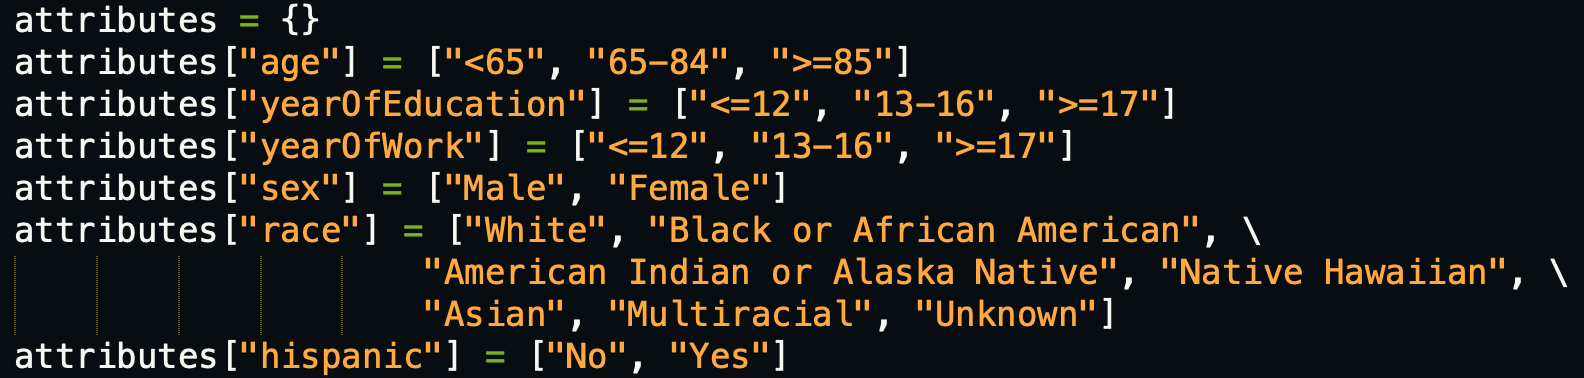
\includegraphics[width=8cm, height=3cm]{figs/demographics.png}
\caption{Items in each attribute of Demographics.}
\label{f:demographics}
\end{figure}





\subsection{Medical Test}
\paragraph{}
The Medical Test table contains two aspects:

\begin{itemize}
  \item Medical scores, such as MMSE (Mini Mental State Examination), HIS (Hachinski ischemic score), etc.
  \item Result of certain medical test, such as CT showing absence of clinically significant focal lesion, etc.
\end{itemize}
\vspace{2mm}
\noindent The attributes in the Medical Test table are shown in Fig.\ref{f:medtest_attr}.

\begin{figure}[!hbt]
\centering
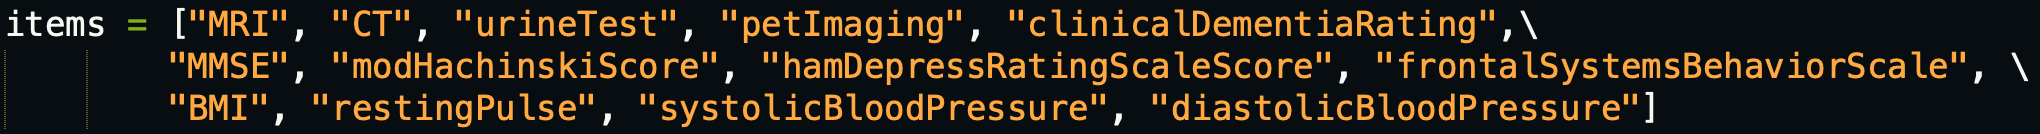
\includegraphics[width=11cm, height=1cm]{figs/medtest_attr.png}
\caption{Attributes of Medical Test.}
\label{f:medtest_attr}
\end{figure}

\noindent Since we do not have the distribution data, the probabilities of each item in this table are self-determined. The items in each attribute are shown in Fig.\ref{f:medtest}.

\begin{figure}[!hbt]
\centering
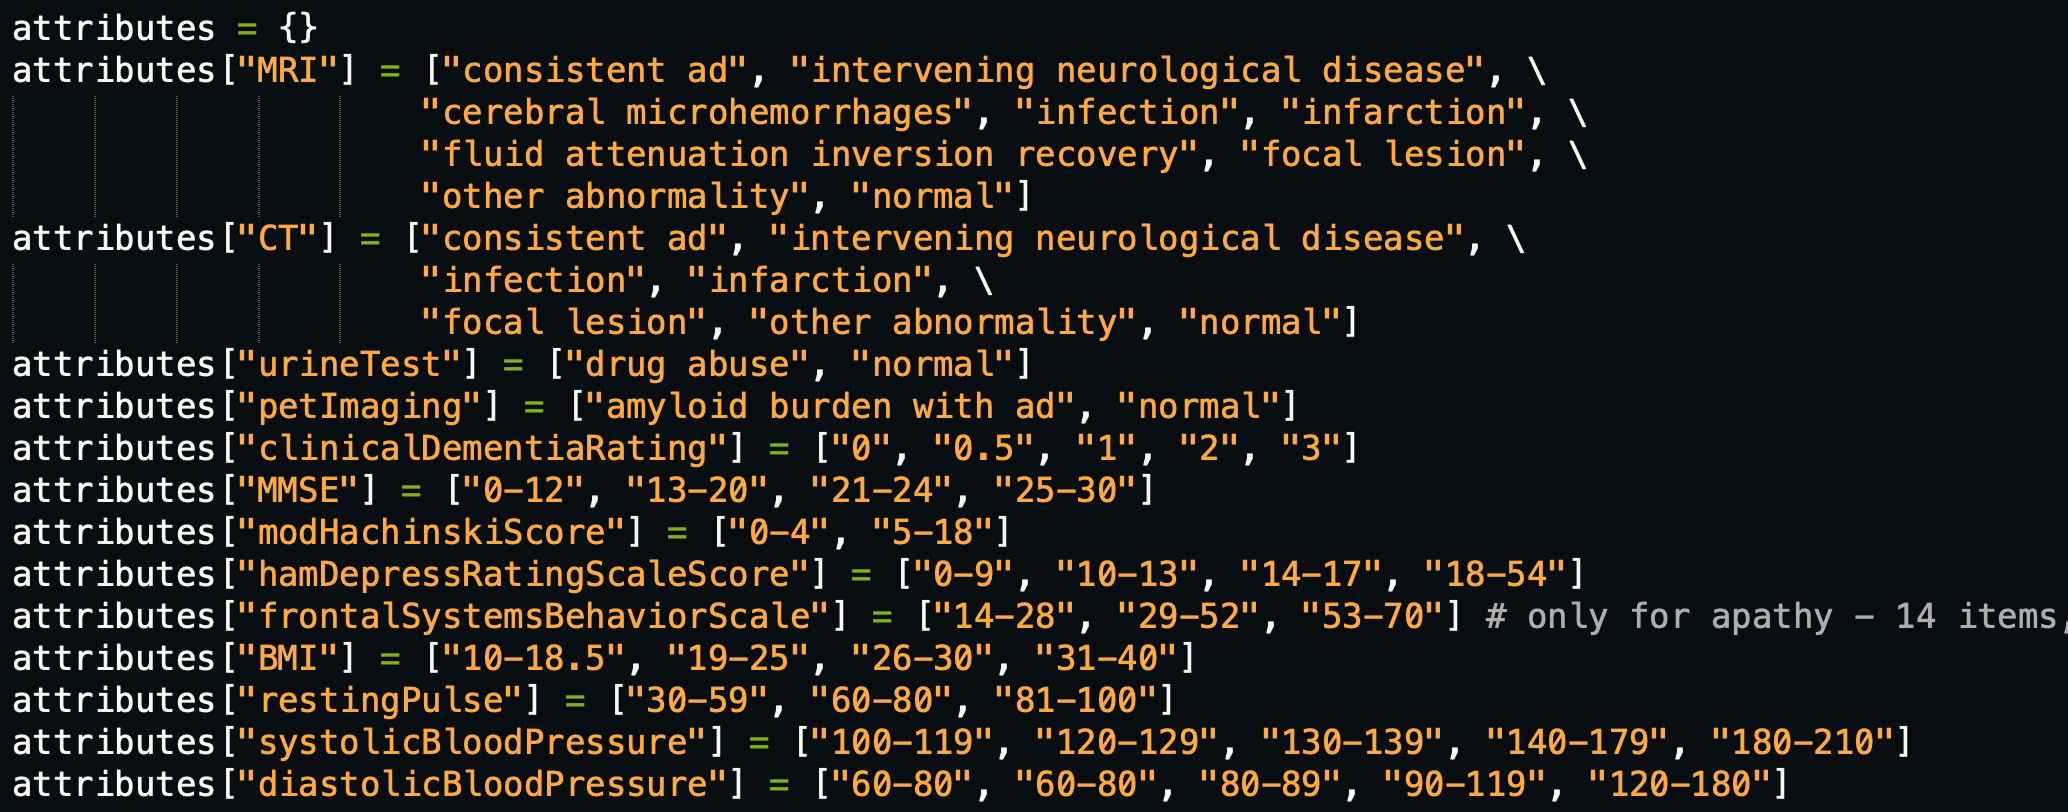
\includegraphics[width=10cm, height=5cm]{figs/medtest.png}
\caption{Items in each attribute of Medical Test.}
\label{f:medtest}
\end{figure}




\subsection{Medical History}
\paragraph{}
The Medical History contains three aspects:

\begin{itemize}
  \item Whether a patient has a certain disease or symptom, such as psychiatric disorders, seizures, etc.
  \item Whether a patient has a certain habit in a period of time, such as smoking, alcohol, etc.
  \item Whether a patient uses a certain medicine in a period of time, such as phenytoin, carbamazepine, etc.
\end{itemize}
\vspace{2mm}
\noindent The attributes in the Medical History table are shown in Fig.\ref{f:medhist_attr}.

\begin{figure}[!hbt]
\centering
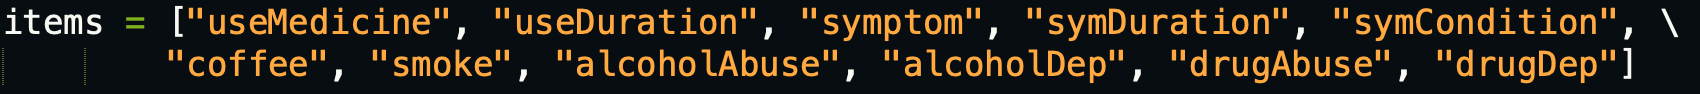
\includegraphics[width=11cm, height=0.8cm]{figs/medhist_attr.png}
\caption{Attributes of Medical History.}
\label{f:medhist_attr}
\end{figure}

\noindent Before showing the attributes in the medical history table, we summarized the types of medicines mentioned in the criteria. Currently, there are 37 types of medicines (Fig.\ref{f:medicine}). The medicine is stored in the Medicine table, where each medicine is assigned with a unique ID. The "useMedicine" attribute in the Medical History table corresponds to each ID in the Medicine table.

\begin{figure}[!hbt]
\centering
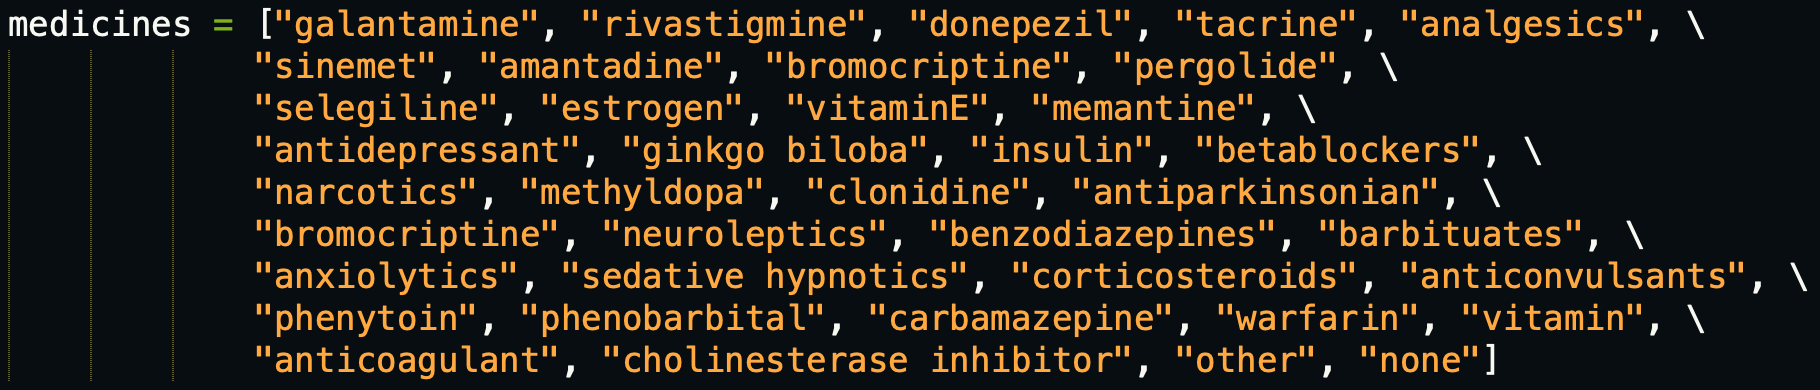
\includegraphics[width=10cm, height=2.5cm]{figs/medicine.png}
\caption{Items in Medicine.}
\label{f:medicine}
\end{figure}

\newpage
\noindent Next, we present the items of each attribute in medical history , Fig.\ref{f:medhistory}. The probabilities of each item of attributes in Medical History are self-determined because of lack of data. \textbf{Note} that the "symptom" and "useMedicine" are not necessarily related with each other. That is, a medicine that a patient takes may not cure for the symptom that the patient has. Moreover, for each sick patient, he may \textbf{at most} have three different symptoms and use three different medicines.

\begin{figure}[!hbt]
\centering
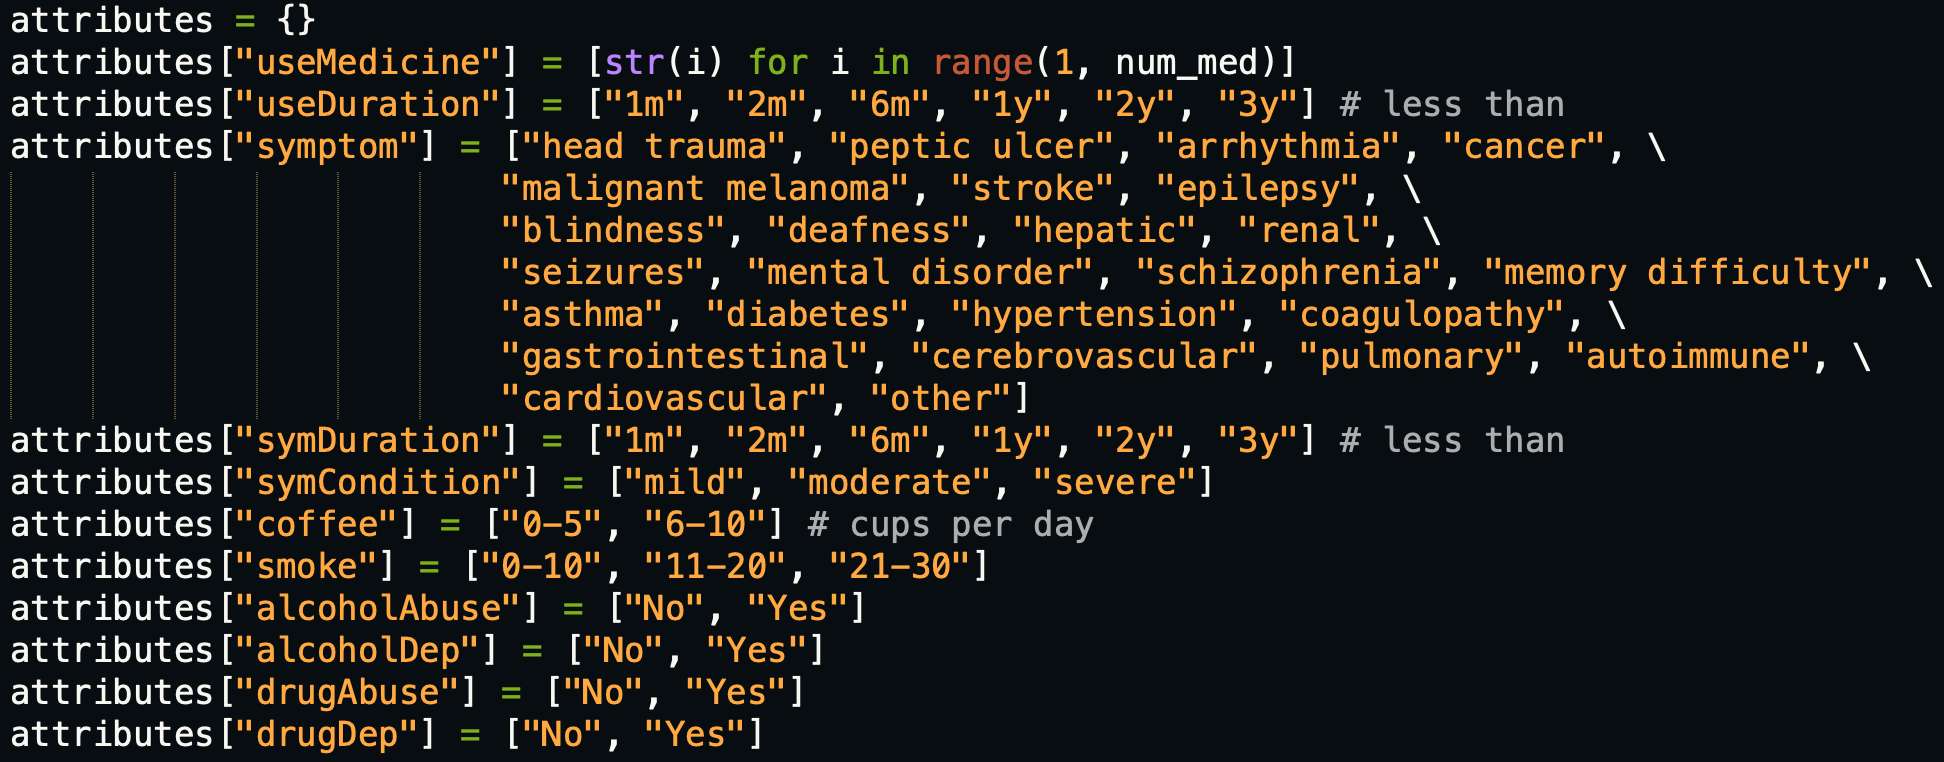
\includegraphics[width=10cm, height=5cm]{figs/medhistory.png}
\caption{Items in each attribute of Medical History.}
\label{f:medhistory}
\end{figure}





\subsection{Personal Characteristics}
\paragraph{}
For the personal characteristics, it mainly contains the willingness, physical ability, caregiver condition and other features:

\begin{itemize}
  \item Personal willingness, such as willingness to visit places, etc.
  \item Personal ability, such as normal ability to speak or understand, etc.
  \item The characteristics of patient's caregiver, such as willingness to accompany the patient, etc.
  \item Other features: disability, presence of metal devices inside body, etc.
\end{itemize}
\vspace{2mm}
\noindent The attributes in the Personal Characteristics table are shown in Fig.\ref{f:personal_attr}.

\begin{figure}[!hbt]
\centering
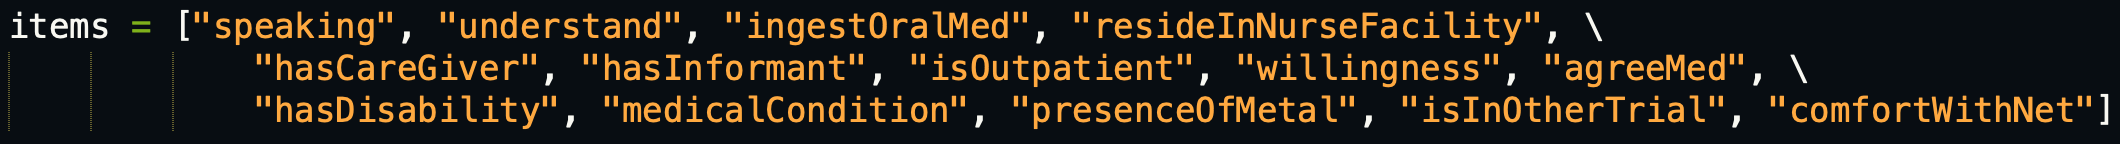
\includegraphics[width=11cm, height=1cm]{figs/personal_attr.png}
\caption{Attributes of Personal Characteristics.}
\label{f:personal_attr}
\end{figure}

\noindent Again, the probabilities of each item in this table are self-determined. The items in each attribute are shown in Fig.\ref{f:personal}.

\begin{figure}[!hbt]
\centering
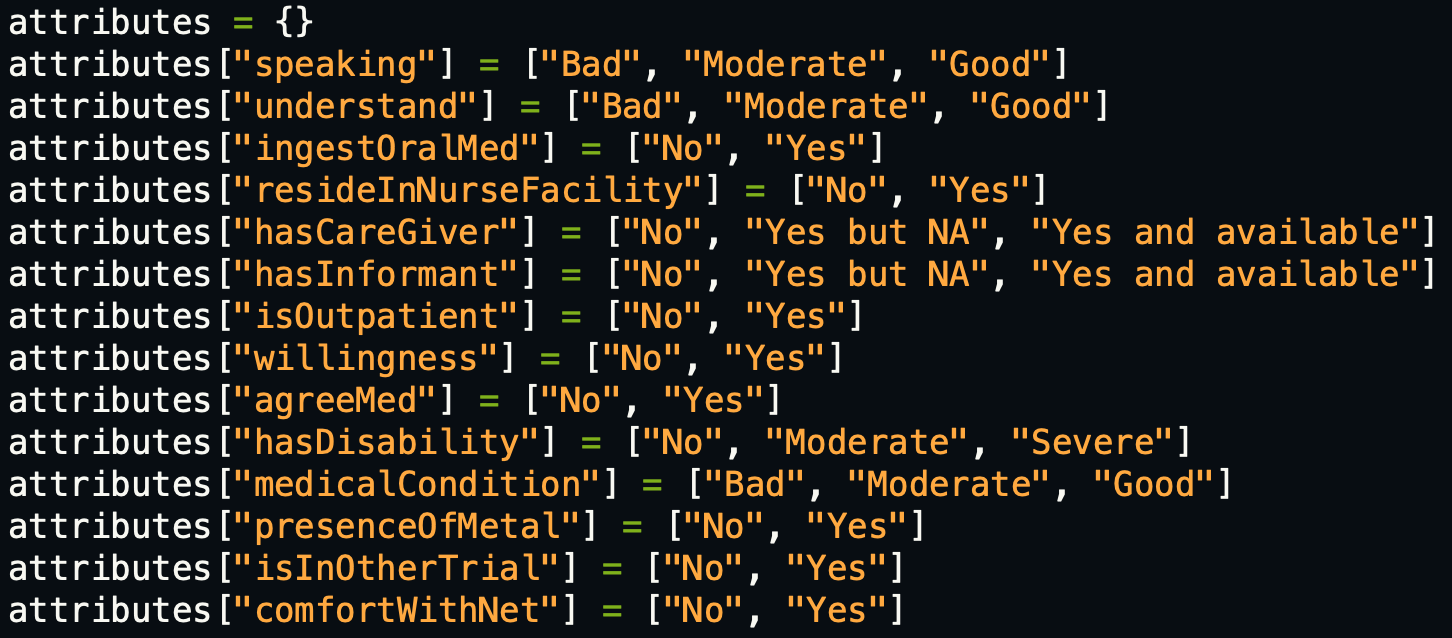
\includegraphics[width=9cm, height=3.5cm]{figs/personal.png}
\caption{Items in each attribute of Personal Characteristics.}
\label{f:personal}
\end{figure}


\newpage
\section{Generated data}
\paragraph{}
Here we randomly generate 10 patients data in the four tables. The results are shown in the following:

\begin{figure}[!hbt]
\centering
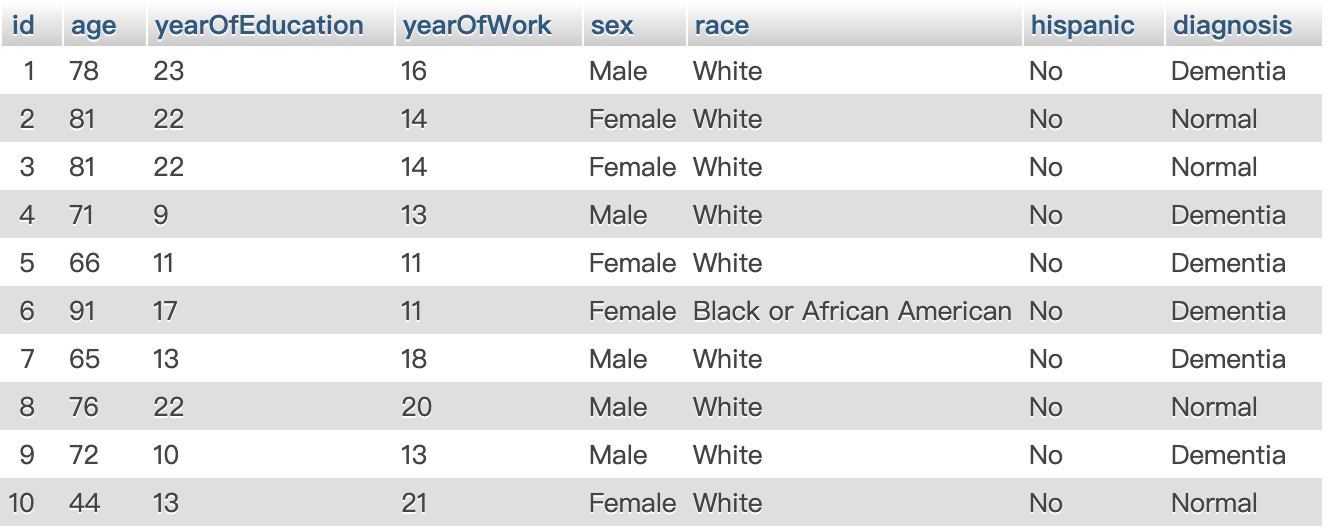
\includegraphics[width=10cm, height=5cm]{figs/res_basics.png}
\caption{Demographics table.}
\label{f:res_basics}
\end{figure}

\begin{figure}[!hbt]
\centering
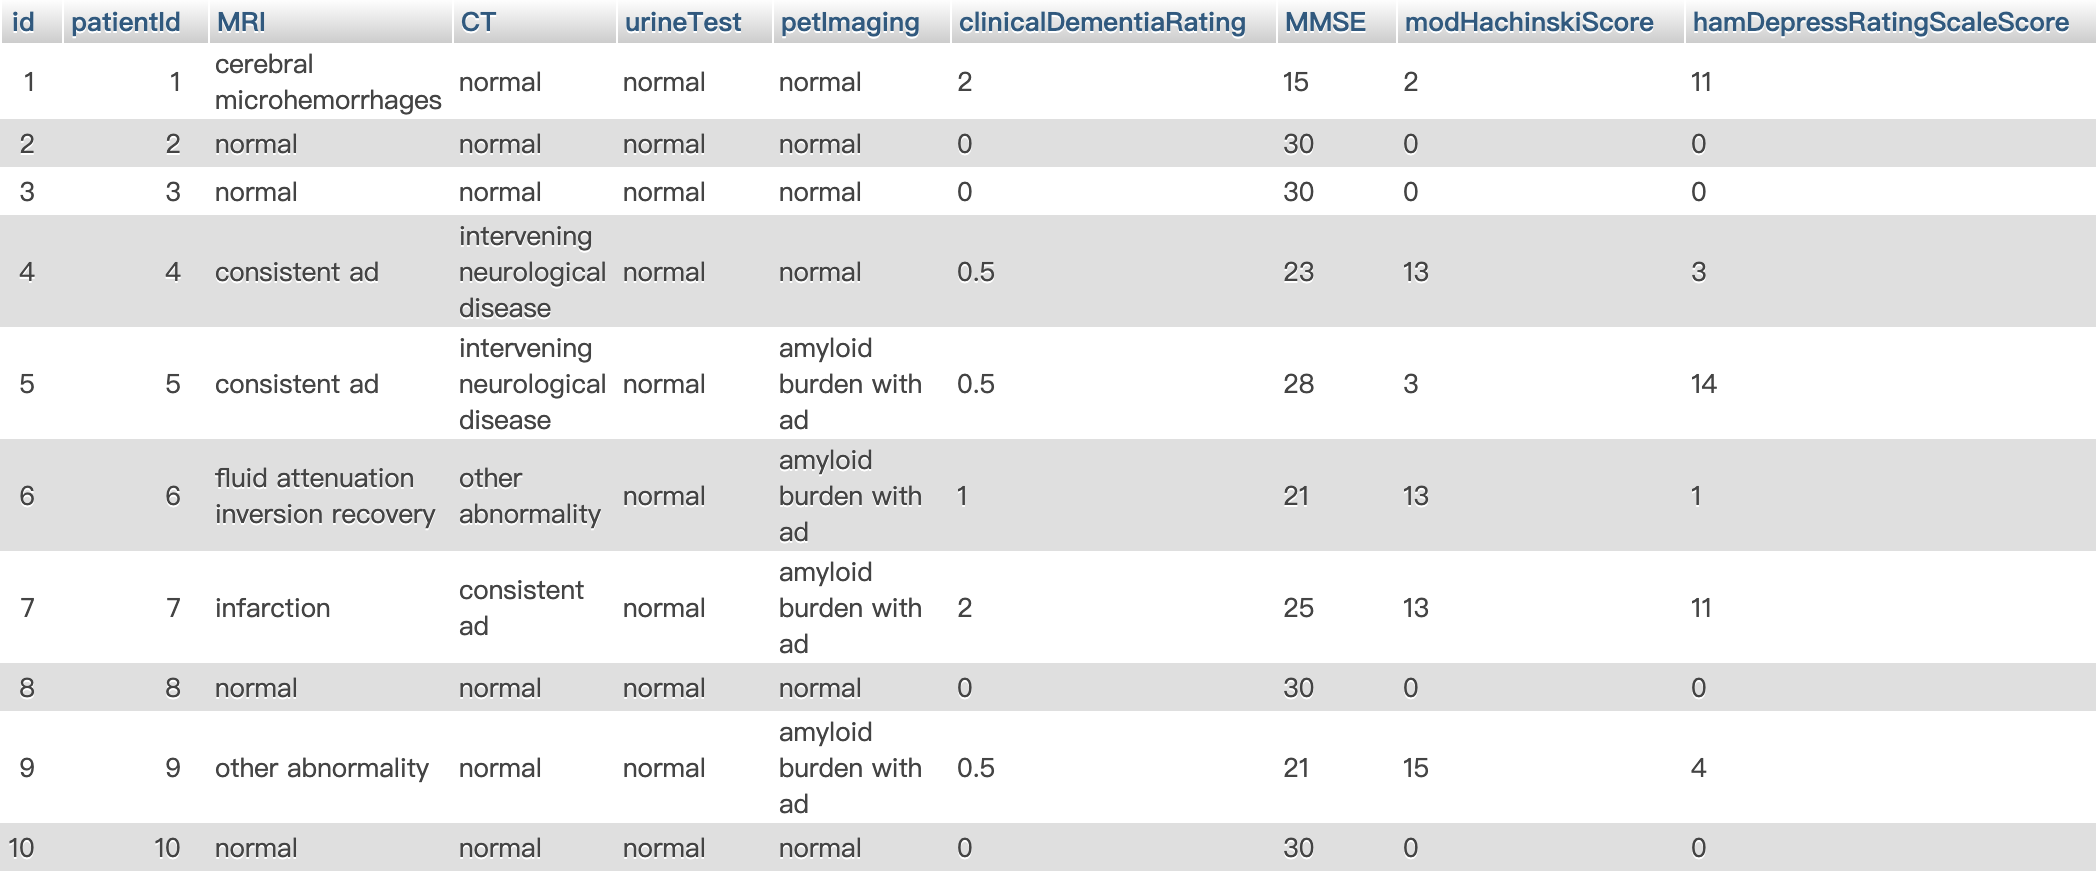
\includegraphics[width=10cm, height=5cm]{figs/res_medtest1.png}
\caption{Medical Test table (part 1).}
\label{f:res_medtest1}
\end{figure}

\begin{figure}[!hbt]
\centering
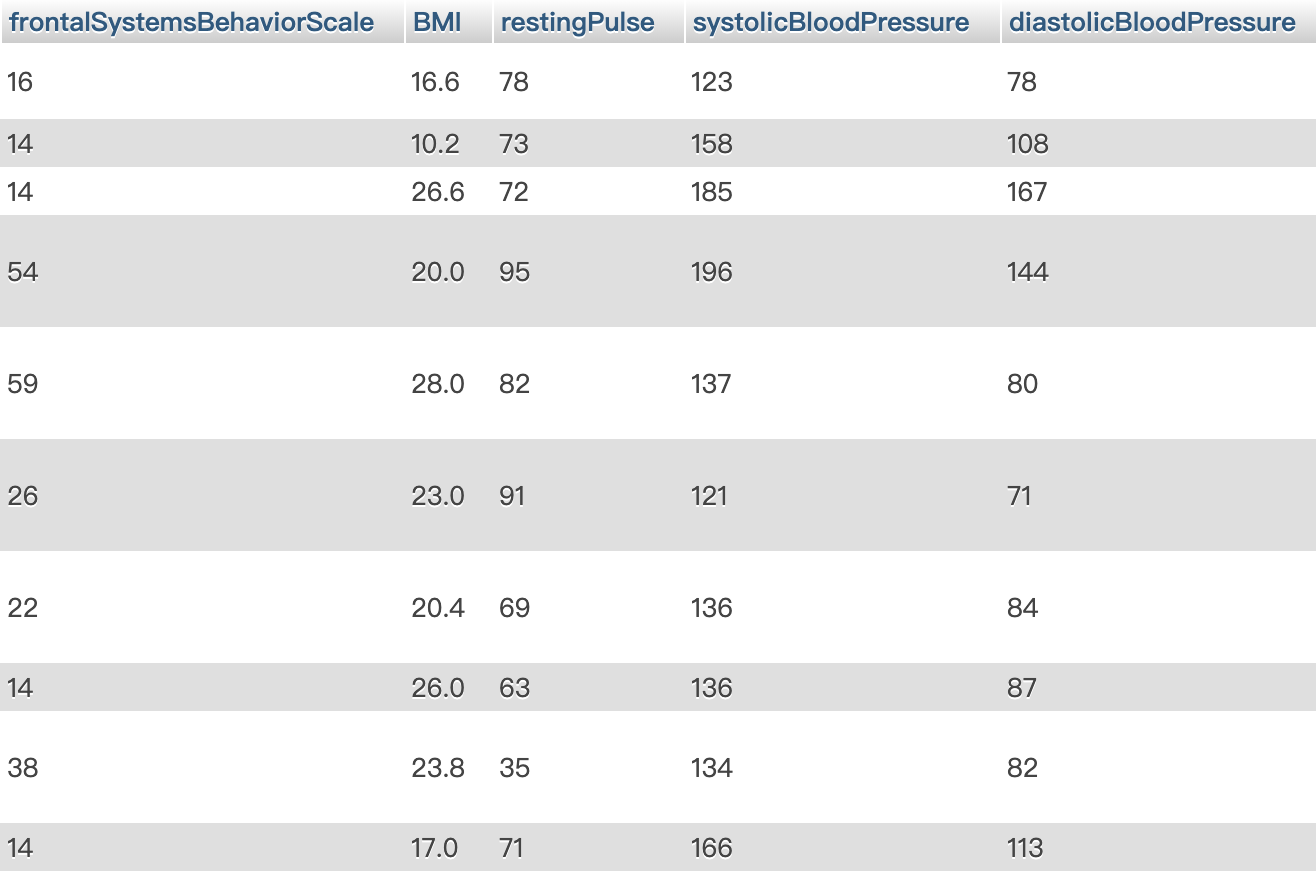
\includegraphics[width=8cm, height=5cm]{figs/res_medtest2.png}
\caption{Medical Test table (part 2).}
\label{f:res_medtest2}
\end{figure}

\begin{figure}[!hbt]
\centering
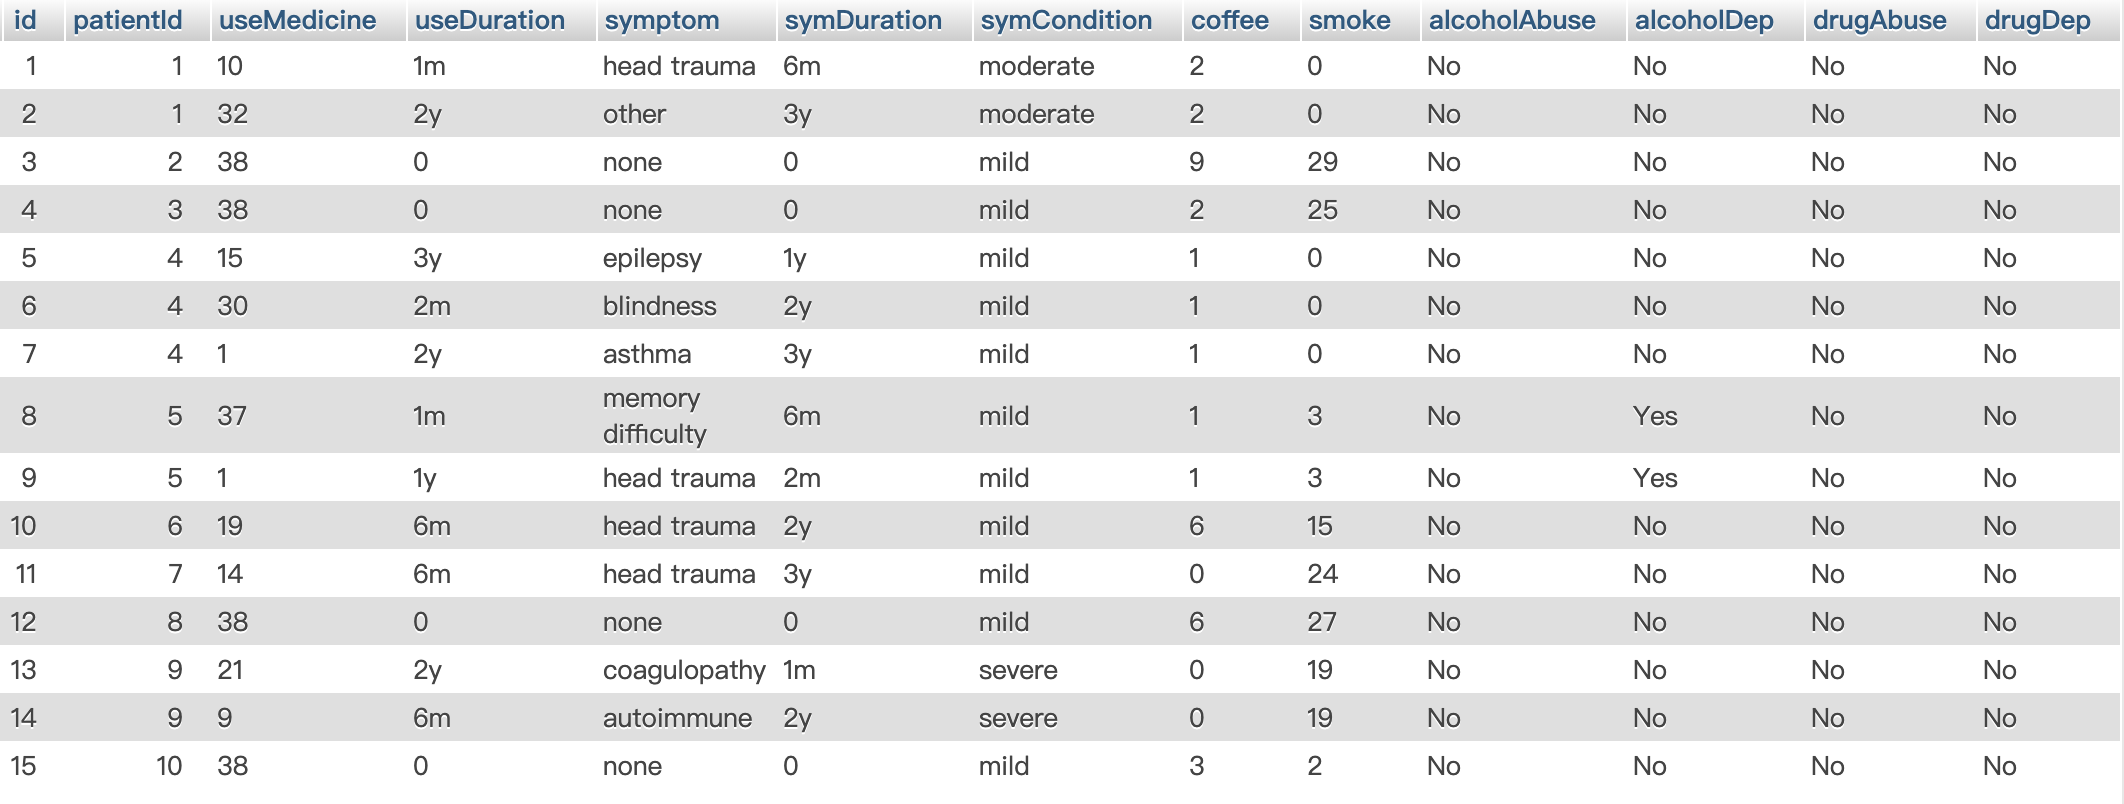
\includegraphics[width=10cm, height=4cm]{figs/res_medhist.png}
\caption{Medical History table.}
\label{f:res_medhist}
\end{figure}

\begin{figure}[!hbt]
\centering
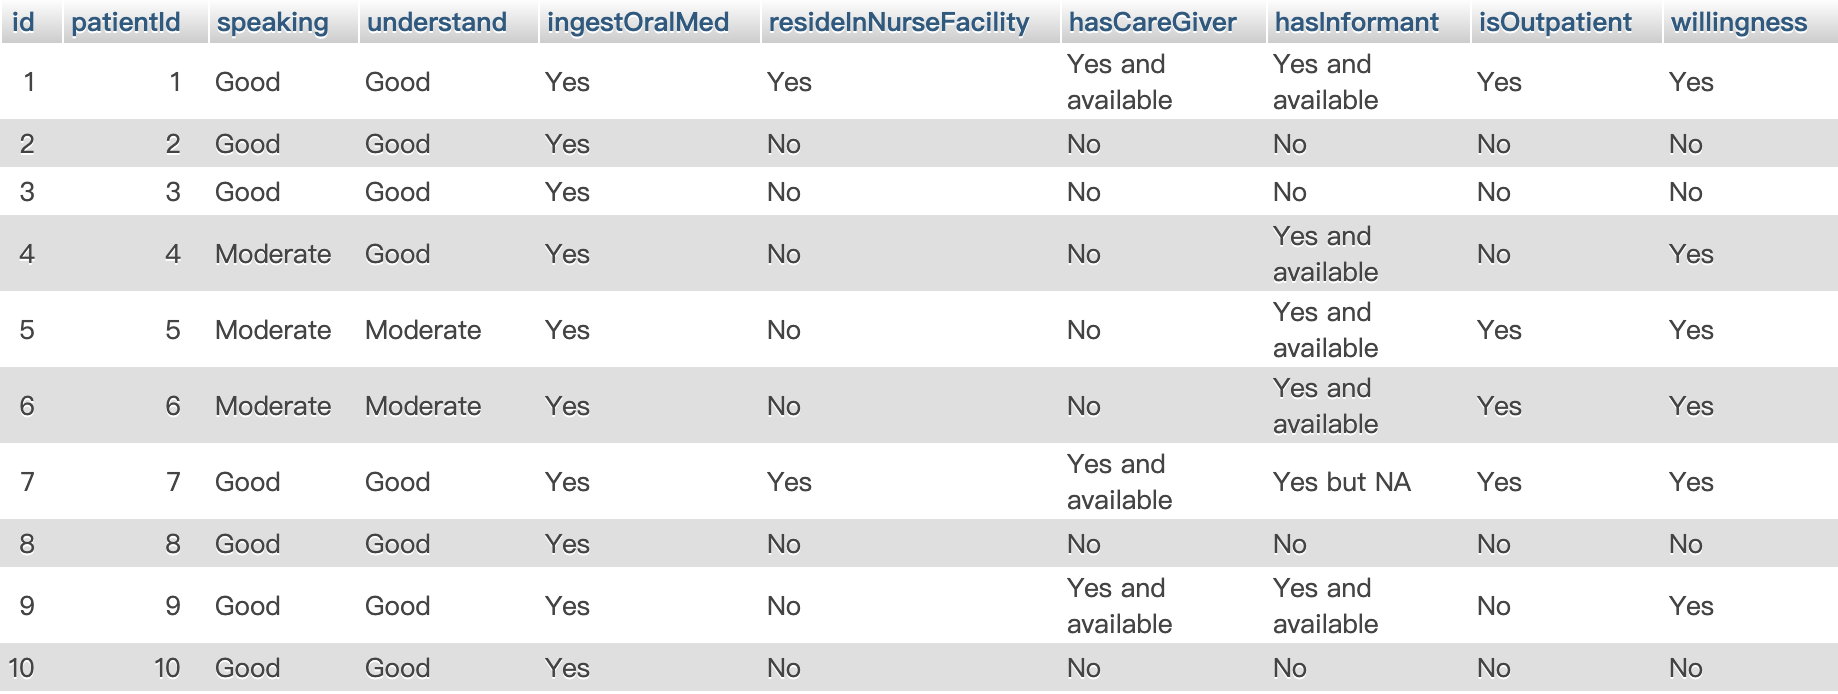
\includegraphics[width=10cm, height=4cm]{figs/res_personal1.png}
\caption{Personal Characteristics table (part 1).}
\label{f:res_personal1}
\end{figure}

\begin{figure}[!hbt]
\centering
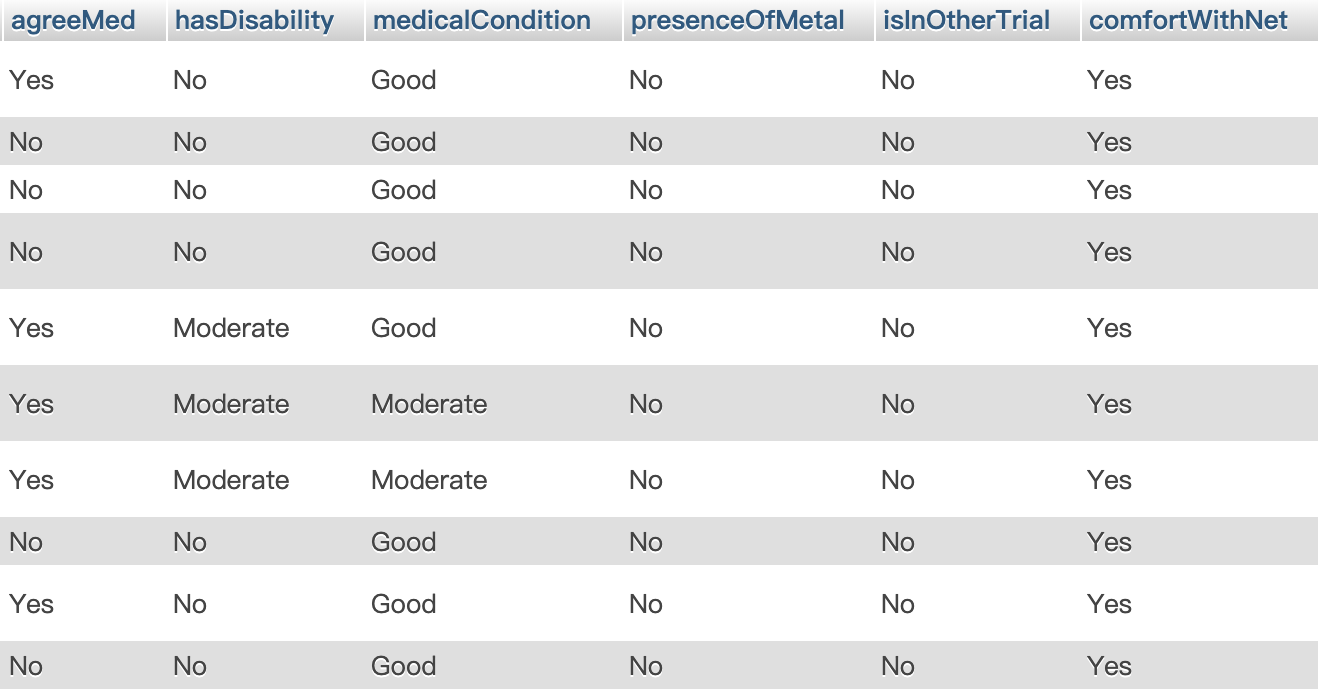
\includegraphics[width=8cm, height=4cm]{figs/res_personal2.png}
\caption{Personal Characteristics table (part 2).}
\label{f:res_personal2}
\end{figure}

\newpage
\section{Issues}
\paragraph{}
There are several issues in the current database:

\begin{itemize}
  \item The probability distributions of items in Medical Test, Medical History and Personal Characteristics are unavailable so far.
  \item The symptom and medicine are not necessarily consistent in Medical History.
  \item Some items may need to be adjusted when the medical data is available.
\end{itemize}




\end{document}












